% Emacs, this is -*-latex-*

\ex{Gram--Schmidt orthogonalisation}
\label{ex:gram-schmidt} 

\begin{exenumerate}
\item Given two vectors $\a_1$ and $\a_2$ in $\mathbb{R}^n$, show that 
  \begin{align}
    \u_1 &= \a_1 \\
    \u_2 &= \a_2 - \frac{\u_1^\top \a_2}{\u_1^\top \u_1}\u_1
  \end{align}
  are orthogonal to each other.
  \begin{solution}
    Two vectors $\u_1$ and $\u_2$ of $\mathbb{R}^n$ are orthogonal
    if their inner product equals zero. Computing the inner product $\u_1^\top \u_2$ gives
    \begin{align}
      \u_1^{\top}\u_2 &= \u_1^\top(\a_2 - \frac{\u_1^\top\a_2}{\u_1^\top\u_1}\u_1) \\
                      &= \u_1^\top\a_2 - \frac{\u_1^\top\a_2}{\u_1^\top\u_1}\u_1^\top\u_1 \\
                      &= \u_1^\top\a_2 - \u_1^\top\a_2 \\
                      &= 0.
    \end{align}
    Hence the vectors $\u_1$ and $\u_2$ are orthogonal.
    
    If $\a_2$ is a multiple of $\a_1$, the orthogonalisation procedure produces
    a zero vector for $\u_2$. To see this, let $\a_2 = \alpha \a_1$ for some
    real number $\alpha$. We then obtain
    \begin{align} \u_2 &= \a_2 - \frac{\u_1^\top \a_2}{\u_1^\top \u_1}\u_1\\
                       &= \alpha \u_1 - \frac{\alpha \u_1^\top \u_1}{\u_1^\top \u_1}\u_1\\
                       &= \alpha \u_1 - \alpha \u_1\\ &=\mathbf{0}.
    \end{align}
  \end{solution}
  
\item Show that any linear combination of (linearly independent) $\a_1$ and $\a_2$ can be written in terms of $\u_1$ and $\u_2$. 
  \begin{solution}
    Let $\v$ be a linear combination of $\a_1$ and $\a_2$, i.e. $\v = \alpha{\a_1} + \beta{\a_2}$ for some real numbers $\alpha$ and $\beta$.
    Expressing $\u_1$ and $\u_2$ in term of $\a_1$ and $\a_2$, we can write $\v$ as
    \begin{align}
      \v  &= \alpha \a_1 + \beta\a_2 \\
          &= \alpha\u_1 + \beta(\u_2 + \frac{\u_1^\top\a_2}{\u_1^\top\u_1}\u_1) \\
          &= \alpha\u_1 + \beta\u_2 + \beta \frac{\u_1^\top\a_2}{\u_1^\top\u_1}\u_1 \\
          &= (\alpha + \beta\frac{\u_1^\top\a_2}{\u_1^\top\u_1})\u_1 + \beta\u_2,
    \end{align}
    Since $\alpha + \beta((\u_1^\top\a_2)/(\u_1^\top\u_1))$ and $\beta$ are real
    numbers, we can write $\v$ as a linear combination of $\u_1$ and
    $\u_2$. Overall, this means that any vector in the span of $\{\a_1, \a_2\}$
    can be expressed in the orthogonal basis $\{\u_1, \u_2\}$.
    
  \end{solution}

\item Show by induction that for any $k \le n$ linearly independent vectors
  $\mathbf{a}_1,\ldots,\mathbf{a}_k$, the vectors $\mathbf{u}_i$, $i=1, \ldots
  k$, are orthogonal, where
  \begin{align}
    \u_i &= \a_i - \sum_{j=1}^{i-1} \frac{\u_j^\top \a_i}{\u_j^\top\u_j} \u_j. \label{eq:Gram-Schmidt-basis-def}
  \end{align}
  The calculation of the vectors $\u_i$ is called Gram–Schmidt orthogonalisation.
  \begin{solution}
   We have shown above that the claim holds for two vectors. This is the base
   case for the proof by induction. Assume now that the claim holds for $k$
   vectors. The induction step in the proof by induction then consists of
   showing that the claim also holds for $k+1$ vectors.
   
   Assume that $\u_1, \u_2, \ldots, \u_k$ are orthogonal vectors. The linear independence assumption ensures that none of the
   $\u_i$ is a zero vector. We then have for $\u_{k+1}$
    \begin{align}
      \u_{k+1} &= \a_{k+1} - \frac{\u_1^\top\a_{k+1}}{\u_1^\top\u_1}\u_1 - \frac{\u_2^\top\a_{k+1}}{\u_2^\top\u_2}\u_2
                 - \ldots - \frac{\u_k^\top\a_{k+1}}{\u_k^\top\u_k}\u_k,
                 \label{eq:u_k+1}
    \end{align}
    and for all $i = 1, 2, \ldots, k$
    \begin{align}
      \u_i^\top\u_{k+1} &= \u_i^\top\a_{k+1} - \frac{\u_1^\top\a_{k+1}}{\u_1^\top\u_1}\u_i^\top\u_1 - 
                          \ldots - \frac{\u_k^\top\a_{k+1}}{\u_k^\top\u_k}\u_i^\top\u_k.
    \end{align}
    By assumption $\u_i^\top\u_j = 0$ if $i \neq j$, so that
    \begin{align}
      \u_i^\top\u_{k+1} &= \u_i^\top\a_{k+1} - 0 - \ldots - \frac{\u_i^\top\a_{k+1}}{\u_i^\top\u_i}\u_i^\top\u_i - 0 \ldots - 0 \\
                        &= \u_i^\top\a_{k+1} - \u_i^\top\a_{k+1} \\
                        &= 0,
    \end{align}
    which means that $\u_{k+1}$ is orthogonal to $\u_1, \ldots, \u_k$.
    
  \end{solution}

\item Show by induction that any linear combination of (linear independent)
  $\a_1, \a_2, \ldots, \a_k$ can be written in terms of $\u_1, \u_2, \ldots,
  \u_k$.
  
  \begin{solution} The base case of two vectors was proved above. Using
    induction, we assume that the claim holds for $k$ vectors and we will prove that
    it then also holds for $k + 1$ vectors: Let $\v$ be a linear combination of
    $\a_1, \a_2, \ldots,
    \a_{k+1}$, i.e. $\v = \alpha_1\a_1 + \alpha_2\a_2 + \ldots + \alpha_k\a_k +
    \alpha_{k+1}\a_{k+1}$ for some real numbers $\alpha_1, \alpha_2, \ldots,
    \alpha_{k+1}$. Using the induction assumption, $\v$ can be written as
    \begin{equation}
      \v = \beta_1\u_1 + \beta_2\u_2 + \ldots + \beta_k\u_k + \alpha_{k+1}\a_{k+1},
    \end{equation}
    for some real numbers $\beta_1, \beta_2, \ldots, \beta_k$ Furthermore, using equation \eqref{eq:u_k+1}, $\v$ can be written as
    \begin{align}
      \v &= \beta_1\u_1  + \ldots + \beta_k\u_k + \alpha_{k+1}\u_{k+1} + \alpha_{k+1}\frac{\u_1^\top\a_{k+1}}{\u_1^\top\u_1}\u_1 \\ 
         &\phantom{=}+ \ldots + \alpha_{k+1}\frac{\u_k^\top\a_{k+1}}{\u_k^\top\u_k}\u_k.
    \end{align}
    With $\gamma_i = \beta_i + \alpha_{k+1}(\u_i^\top\a_{k+1})/(\u_i^\top\u_i)$, $\v$ can thus be written as
    \begin{align}
      \v &= \gamma_1\u_1 + \gamma_2\u_2 + \ldots + \gamma_k\u_k + \alpha_{k+1}\u_{k+1},
    \end{align}
    which completes the proof. Overall, this means that the $\u_1, \u_2, \ldots,
    \u_k$ form an orthogonal basis for $\text{span}(\a_1, \ldots, \a_k)$, i.e.\
    the set of all vectors that can be obtained by linearly combining the
    $\a_i$.

  \end{solution}
  
\item Consider the case where $\a_1, \a_2, \ldots, \a_k$ are linearly
  independent and $\a_{k+1}$ is a linear combination of $\a_1, \a_2, \ldots,
  \a_k$. Show that $\u_{k+1}$, computed according to
  \eqref{eq:Gram-Schmidt-basis-def}, is zero.

  \begin{solution}
    Starting with \eqref{eq:Gram-Schmidt-basis-def}, we have
    \begin{equation}
      \u_{k+1} = \a_{k+1} - \sum_{j=1}^{k} \frac{\u_j^\top \a_{k+1}}{\u_j^\top\u_j} \u_j.
    \end{equation}
    By assumption, $\a_{k+1}$ is a linear combination of $\a_1, \a_2, \ldots,
    \a_k$. By the previous question, it can thus also be written as a linear
    combination of the $\u_1, \ldots, \u_k$. This means that there are some
    $\beta_i$ so that
    \begin{equation}
      \a_{k+1} = \sum_{i=1}^k \beta_i \u_i
    \end{equation}
    holds. Inserting this expansion into the equation above gives
    \begin{align}
      \u_{k+1}  &=  \sum_{i=1}^k \beta_i \u_i - \sum_{j=1}^k \sum_{i=1}^k \beta_i \frac{\u_j^\top\u_i}{\u_j^\top\u_j} \u_j\\
                &= \sum_{i=1}^k \beta_i \u_i - \sum_{i=1}^k \beta_i  \frac{\u_i^\top\u_i}{\u_i^\top\u_i} \u_i
    \end{align}
    because $\u_j^\top \u_i =0$ if $i \neq j$. We thus obtain the desired result:
    \begin{align}
      \u_{k+1} & =  \sum_{i=1}^k \beta_i \u_i - \sum_{i=1}^k \beta_i \u_i\\
               &= 0
    \end{align}
    This property of the Gram-Schmidt process in
    \eqref{eq:Gram-Schmidt-basis-def} can be used to check whether a list of
    vectors $\a_1, \a_2, \ldots, \a_d$ is linearly independent or not. If, for
    example, $\u_{k+1}$ is zero, $\a_{k+1}$ is a linear combination of the $\a_1,
    \ldots, \a_k$. Moreover, the result can be used to extract a sublist of linearly
    independent vectors: We would remove $\a_{k+1}$ from the list and restart
    the procedure in \eqref{eq:Gram-Schmidt-basis-def} with $\a_{k+2}$ taking
    the place of $\a_{k+1}$. Continuing in this way constructs a list of
    linearly independent $\a_j$ and orthogonal $\u_j$, $j=1, \ldots, r$, where
    $r$ is the number of linearly independent vectors among the $\a_1, \a_2,
    \ldots, \a_d$.

  \end{solution}
\end{exenumerate}

% --------------------------------------------------
\ex{Linear transforms}
\label{ex:linear-transforms}

\begin{exenumerate}
\item Assume two vectors $ \a_1$ and $\a_2$ are in $\mathbb{R}^2$. Together,
  they span a parallelogram. Use \exref{ex:gram-schmidt} to show that the
  squared area $S^2$ of the parallelogram is given by
  \begin{equation}
    S^2 = (\a_2^T\a_2)(\a_1^T\a_1)-(\a_2^T\a_1)^2
  \end{equation}
  
  \begin{solution}
    Let $\a_1$ and $\a_2$ be the vectors that span the parallelogram. From geometry we
    know that the area of parallelogram is base times height, which is
    equivalent to the length of the base vector times the length of the height vector.
    Denote this by $S^2 = ||\a_1||^2||\u_2||^2$, where is $\a_1$ is the base
    vector and $\u_2$ is the height vector which is orthogonal to the base
    vector. Using the Gram--Schmidt process for the vectors $\a_1$ and $\a_2$ in that
    order, we obtain the vector $\u_2$ as the second  output.
    % 
    \begin{figure}[h!]
      \centering
      \scalebox{0.75}{
        \input{figs/linear-algebra/gram.pstex_t} }
    \end{figure}
    
    Therefore $||\u_2||^2$ equals
    \begin{align}
      ||\u_2||^2 &= \u_2^\top\u_2 \\
                 &= \left(\a_2 - \frac{\a_1^\top\a_2}{\a_1^\top\a_1}\a_1\right)^\top\left(\a_2 - \frac{\a_1^\top\a_2}{\a_1^\top\a_1}\a_1\right) \\
                 &= \a_2^\top\a_2 - \frac{(\a_1^\top\a_2)^2}{\a_1^\top\a_1} - \frac{(\a_1^\top\a_2)^2}{\a_1^\top\a_1} + \left(\frac{\a_1^\top\a_2}{\a_1^\top\a_1}\right)^2\a_1^\top\a_1 \\
                 &= \a_2^\top\a_2 - \frac{(\a_1^\top\a_2)^2}{\a_1^\top\a_1}.
    \end{align}
    Thus, $S^2$ is:
    \begin{align}
      S^2 &= ||\a_1||^2||\u_2||^2 \\
          &= (\a_1^\top\a_1)(\u_2^\top\u_2) \\
          &= (\a_1^\top\a_1)\left(\a_2^\top\a_2 - \frac{(\a_1^\top\a_2)^2}{\a_1^\top\a_1}\right) \\
          &= (\a_2^\top\a_2)(\a_1^\top\a_1) - (\a_1^\top\a_2)^2.
    \end{align}

  \end{solution}
  
\item Form the matrix $\A=(\a_1 \; \a_2)$ where $\a_1$ and $\a_2$ are
  the first and second column vector, respectively. Show that
  \begin{equation}
    S^2 = (\det \A)^2.
  \end{equation}
  
  
  \begin{solution}
    We form the matrix $\A$,
    \begin{equation}
      \A = \begin{pmatrix} \a_1 & \a_2
           \end{pmatrix}  =
           \begin{pmatrix} a_{11} & a_{12} \\ a_{21} & a_{22}
           \end{pmatrix}.
    \end{equation}
    The determinant of $\A$ is $\det \A = a_{11}a_{22} - a_{12}a_{21}$. By multiplying out $(\a_2^\top\a_2)$, $(\a_1^\top\a_1)$ and 
    $(\a_1^\top\a_2)^2$, we get
    \begin{align}
      \a_2^\top\a_2 	&= a_{12}^2 + a_{22}^2 \\ 
      \a_1^\top\a_1 	&= a_{11}^2 + a_{21}^2 \\
      (\a_1^\top\a_2)^2 	&= (a_{11}a_{12} + a_{21}a_{22})^2 = a_{11}^2a_{12}^2 + a_{21}^2a_{22}^2 + 2a_{11}a_{12}a_{21}a_{22}.
    \end{align}
    Therefore the area equals
    \begin{align}
      S^2 &= (a_{12}^2 + a_{22}^2)(a_{11}^2 + a_{21}^2) - (\a_1^\top\a_2)^2 \\
          &= a_{12}^2a_{11}^2 + a_{12}^2a_{21}^2 + a_{22}^2a_{11}^2 + a_{22}^2a_{21}^2 \nonumber\\
          &\phantom{=}- (a_{12}^2a_{11}^2 + a_{21}^2a_{22}^2 + 2a_{11}a_{12}a_{21}a_{22}) \\
          &= a_{12}^2a_{21}^2 + a_{22}^2a_{11}^2 - 2a_{11}a_{12}a_{21}a_{22} \\
          &= (a_{11}a_{22} - a_{12}a_{21})^2,
    \end{align}
    which equals $(\det \A)^2$.
  \end{solution}
\item Consider the linear transform $\y=\A\x$ where $\A$
  is a $2 \times 2$ matrix. Denote the image of the rectangle $U_x=[x_1 \;
  x_1+\triangle_1]\times [x_2 \; x_2+\triangle_2]$ under the transform
  $\A$ by $U_y$. What is $U_y$? What is the area of $U_y$?
  
  \begin{solution} $U_y$ is parallelogram that is spanned by the column
    vectors $\a_1$ and $\a_2$ of $\A$, when $\A = (\a_1 \; \a_2)$.
    
    A rectangle with the same area as $U_x$ is spanned by vectors $(\Delta_1,
    0)$ and $(0, \Delta_2)$. Under the linear transform $\A$ these spanning
    vectors become $\Delta_1\a_1$ and $\Delta_2\a_2$. Therefore a parallelogram
    with the same area as $U_y$ is spanned by $\Delta_1\a_1$ and
    $\Delta_2\a_2$ as shown in the following figure.
    \begin{figure}[htp] \centering \scalebox{0.4}{
        \begin{picture}(0,0)%
          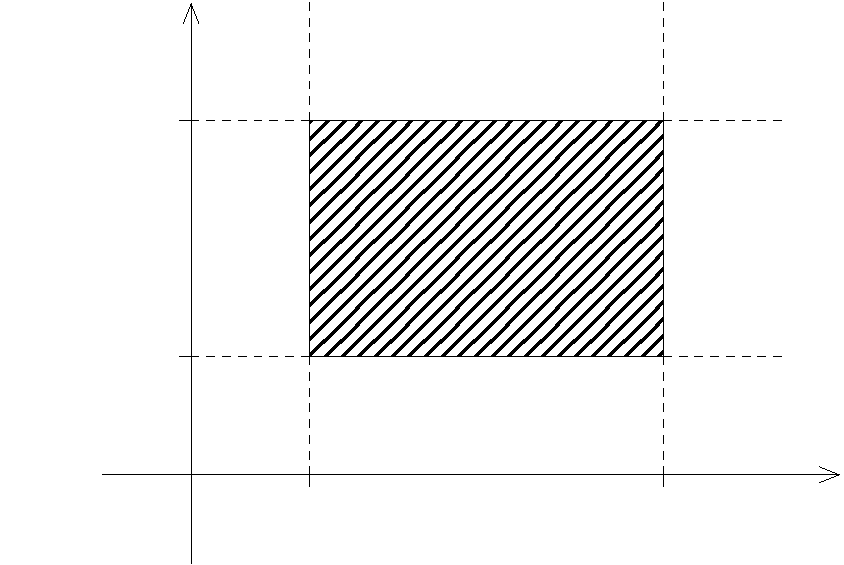
\includegraphics{linear1.pdf}%
        \end{picture}%
        \setlength{\unitlength}{4144sp}%
        % 
        \begingroup\makeatletter\ifx\SetFigFont\undefined%
          \gdef\SetFigFont#1#2#3#4#5{%
            \reset@font\fontsize{#1}{#2pt}%
            \fontfamily{#3}\fontseries{#4}\fontshape{#5}%
            \selectfont}%
        \fi\endgroup%
        \begin{picture}(6417,4299)(-1454,152)
          \put(2026,3809){\makebox(0,0)[lb]{\smash{{\SetFigFont{25}{30.0}{\familydefault}{\mddefault}{\updefault}{\color[rgb]{0,0,0}$U_x$}%
                }}}}
          \put(-629,1649){\makebox(0,0)[lb]{\smash{{\SetFigFont{25}{30.0}{\familydefault}{\mddefault}{\updefault}{\color[rgb]{0,0,0}$x_2$}%
                }}}}
          \put(3016,434){\makebox(0,0)[lb]{\smash{{\SetFigFont{25}{30.0}{\familydefault}{\mddefault}{\updefault}{\color[rgb]{0,0,0}$x_1 + \Delta_1$}%
                }}}}
          \put(-1439,3449){\makebox(0,0)[lb]{\smash{{\SetFigFont{25}{30.0}{\familydefault}{\mddefault}{\updefault}{\color[rgb]{0,0,0}$x_2 + \Delta_2$}%
                }}}}
          \put(721,434){\makebox(0,0)[lb]{\smash{{\SetFigFont{25}{30.0}{\familydefault}{\mddefault}{\updefault}{\color[rgb]{0,0,0}$x_1$}%
                }}}}
        \end{picture}%
      }
      % 
      \scalebox{0.4}{ 
        \begin{picture}(0,0)%
          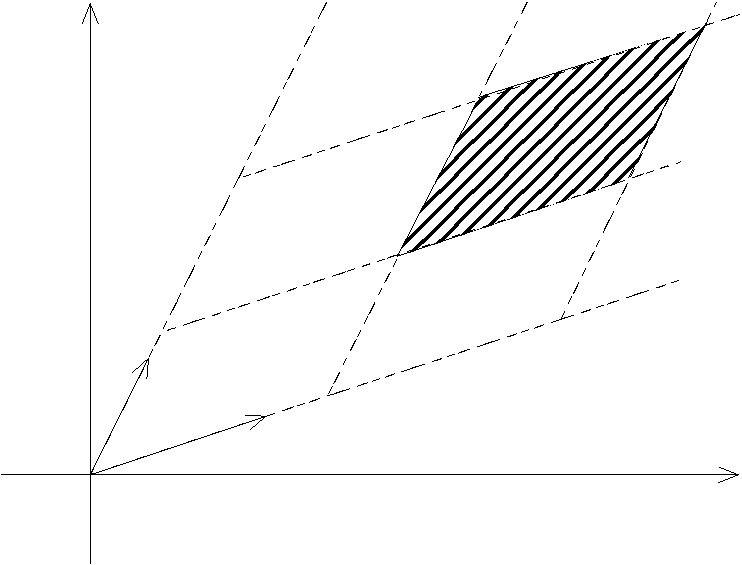
\includegraphics{linear2.pdf}%
        \end{picture}%
        \setlength{\unitlength}{4144sp}%
        % 
        \begingroup\makeatletter\ifx\SetFigFont\undefined%
          \gdef\SetFigFont#1#2#3#4#5{%
            \reset@font\fontsize{#1}{#2pt}%
            \fontfamily{#3}\fontseries{#4}\fontshape{#5}%
            \selectfont}%
        \fi\endgroup%
        \begin{picture}(5649,4299)(-686,152)
          \put(1711,1199){\makebox(0,0)[lb]{\smash{{\SetFigFont{17}{20.4}{\familydefault}{\mddefault}{\updefault}{\color[rgb]{0,0,0}$x_1$}%
                }}}}
          \put(3241,1694){\makebox(0,0)[lb]{\smash{{\SetFigFont{17}{20.4}{\familydefault}{\mddefault}{\updefault}{\color[rgb]{0,0,0}$x_1 + \Delta_1$}%
                }}}}
          \put( 91,3044){\makebox(0,0)[lb]{\smash{{\SetFigFont{17}{20.4}{\familydefault}{\mddefault}{\updefault}{\color[rgb]{0,0,0}$x_2 + \Delta_2$}%
                }}}}
          \put(181,1874){\makebox(0,0)[lb]{\smash{{\SetFigFont{17}{20.4}{\familydefault}{\mddefault}{\updefault}{\color[rgb]{0,0,0}$x_2$}%
                }}}}
          \put(991,929){\makebox(0,0)[lb]{\smash{{\SetFigFont{20}{24.0}{\familydefault}{\mddefault}{\updefault}{\color[rgb]{0,0,0}$\mathbf{a}_1$}%
                }}}} 
          \put(406,1289){\makebox(0,0)[lb]{\smash{{\SetFigFont{20}{24.0}{\familydefault}{\mddefault}{\updefault}{\color[rgb]{0,0,0}$\mathbf{a}_2$}%
                }}}}
          \put(3691,4214){\makebox(0,0)[lb]{\smash{{\SetFigFont{25}{30.0}{\familydefault}{\mddefault}{\updefault}{\color[rgb]{0,0,0}$U_y$}%
                }}}}
        \end{picture}%
      }
    \end{figure}
         
    From the previous question, the $A_{U_y}$ of $U_y$ equals the absolute value of the determinant of the matrix $(\Delta_1\a_1 \; \Delta_2\a_2)$:
    \begin{align}
      A_{U_y} &= |\det \begin{pmatrix} \Delta_1a_{11} & \Delta_2a_{12} \\ \Delta_1a_{21} & \Delta_2a_{22} \end{pmatrix} |\\
              &= |\Delta_1\Delta_2a_{11}a_{22} - \Delta_1\Delta_2a_{12}a_{21}| \\ 
              &= |\Delta_1\Delta_2(a_{11}a_{22} - a_{12}a_{21})| \\
              &= \Delta_1\Delta_2 |\det \A|
    \end{align}
    Therefore the area of $U_y$ is the area of $U_x$ times $|\det \A$|.
  \end{solution}
  
\item Give an intuitive explanation why we have equality in the change of variables formula 
  \begin{equation} \int_{U_y} f(\y)d\y = \int_{U_x} f(\A \x) |\det \A| d\x.
  \end{equation} where $\A$ is such that $U_x$ is an axis-aligned (hyper-)
  rectangle as in the previous question.
  
  \begin{solution} We can think that, loosely speaking, the two integrals
    are limits of the following two sums
    \begin{equation} \sum_{\y_i \in U_y}
      f(\y_i) \textrm{vol}(\Delta_{\y_i}) \quad \quad \quad \sum_{\x_i \in U_x}
      f(\A \x_i) |\det \A| \textrm{vol}(\Delta_{\x_i})
    \end{equation}
    where $\x_i = \A^{-1} \y_i$, which means that $\x$ and $\y$ are related
    by $\y = \A \x$. The set of function values $f(\y_i)$ and $f(\A \x_i)$
    that enter the two sums are exactly the same. The volume
    $\textrm{vol}(\Delta_{\x_i})$ of a small axis-aligned hypercube (in $d$
    dimensions) equals $\prod_{i=1}^d \Delta_i$. The image of this small
    axis-aligned hypercube under $\A$ is a parallelogram $\Delta_{\y_i}$
    with volume $\textrm{vol}(\Delta_{\y_i})= |\det \A|
    \textrm{vol}(\Delta_{\x_i})$. Hence
    \begin{equation}
      \sum_{\y_i \in U_y} f(\y_i) \textrm{vol}(\Delta_{\y_i}) = \sum_{\x_i \in U_x} f(\A \x_i) |\det \A| \textrm{vol}(\Delta_{\x_i}).
    \end{equation}
    We must have the term $|\det \A|$ to compensate for the fact that the volume of $U_x$ and $U_y$ are not the same. For example, let $\A$ be a diagonal matrix $\diag(10, 100)$ so that $U_x$ is much smaller than $U_y$. The determinant $\det \A = 1000$ then compensates for the fact that the $\x_i$ values are more condensed than the $\y_i$.
  \end{solution}
  
\end{exenumerate}
     

% --------------------------------------------------

\ex{Eigenvalue decomposition}
\label{ex:eigenvalue-decomposition}
For a square matrix $\A$ of size $n \times n$, a vector $\u_i
\neq 0$ which satisfies
\begin{equation}
  \A\u_i = \lambda_i \u_i
  \label{eq:eigenvector}
\end{equation}
is called a eigenvector of $\A$, and $\lambda_i$ is the corresponding
eigenvalue. For a matrix of size $n \times n$, there are $n$
eigenvalues $\lambda_i$ (which are not necessarily distinct).
\begin{exenumerate}
\item Show that if $\u_1$ and $\u_2$ are eigenvectors with $\lambda_1=\lambda_2$, then
  $\u = \alpha \u_1 +\beta \u_2$ is also an eigenvector with the same eigenvalue.
  \begin{solution}
    We compute
    \begin{align}
      \A\u &= \alpha \A\u_1 + \beta \A\u_2 \\
           &= \alpha \lambda \u_1 + \beta \lambda \u_2 \\
           &= \lambda(\alpha\u_1 + \beta\u_2) \\
           &= \lambda \u,
    \end{align}
    so $\u$ is an eigenvector of $\A$ with the same eigenvalue as $\u_1$ and $\u_2$.
  \end{solution}

\item Assume that none of the eigenvalues of $\A$ is zero. Denote by $\U$
  the matrix where the column vectors are linearly independent eigenvectors
  $\u_i$ of $\A$. Verify that \eqref{eq:eigenvector} can be written in matrix form as $\A\U=\U\Lambdab$, where $\Lambdab$ is a
  diagonal matrix with the eigenvalues $\lambda_i$ as diagonal elements.
 
  \begin{solution}
    By basic properties of matrix multiplication, we have
    \begin{align}
      \A\U &= (\A\u_1 \; \A\u_2 \;\ldots \; \A\u_n)
    \end{align}
    With $\A\u_i =\lambda_i \u_i$ for all $i = 1, 2, \ldots, n$, we thus obtain
    \begin{align}
      \A\U & = (\lambda_1\u_1 \; \lambda_2\u_2 \;\ldots \; \lambda_n\u_n) \\
           &= \U\Lambdab.
    \end{align}
  \end{solution}
  
\item Show that we can write, with $\V^T=\U^{-1}$,
  \begin{align}
    \A &= \U \Lambdab \V^\top,&     \A &= \sum_{i=1}^n \lambda_i \u_i\v_i^T,\\
    \A^{-1} &= \U \Lambdab^{-1} \V^\top, & \A^{-1} &= \sum_{i=1}^n \frac{1}{\lambda_i} \u_i\v_i^\top,
  \end{align}
  where $\v_i$ is the $i$-th column of $\V$.
  \begin{solution}
    \begin{enumerate}
    \item[(i)] Since the columns of $\U$ are linearly independent,
      $\U$ is invertible. Because $\A\U = \U\Lambdab$, multiplying from
      the right with the inverse of $\U$ gives $\A = \U\Lambdab \U^{-1} =
      \U\Lambda \V^\top$.
    \item[(ii)] Denote by $\u^{[i]}$ the $i$th row of $\U$,
      $\v^{(j)}$ the $j$th column of $\V^\top$ and $\v^{[j]}$
      the $j$th row of $\V$ and denote $\B = \sum_{i=1}^n
      \lambda_i\u_i\v_i^\top$. Let $\e^{[i]}$ be a row vector
      with 1 in the $i$th place and 0 elsewhere and $\e^{(j)}$ be a
      column vector with 1 in the $j$th place and 0
      elsewhere. Notice that because $\A = \U\Lambdab \V^\top$,
      the element in the $i$th row and $j$th column is
      \begin{align}
        A_{ij}  &= \u^{[i]}\Lambdab \v^{(j)} \\
                &= \u^{[i]}\Lambdab {\v^{[j]}}^\top \\
                &= \u^{[i]} \left( \begin{matrix} \lambda_1V_{j1} \\ \vdots \\ \lambda_nV_{jn} \end{matrix} \right) \\
                &= \sum_{k=1}^n \lambda_k V_{jk}U_{ik}.
      \end{align}
      On the other hand, for matrix $\B$ the element in the $i$th row and $j$th column is
      \begin{align}
        B_{ij}  &= \sum_{k=1}^n \lambda_k\e^{[i]}\u_k\v_k^\top \e^{(j)} \\
                &= \sum_{k=1}^n \lambda_kU_{ik}V_{jk},
      \end{align}
      which is the same as $A_{ij}$. Therefore $\A = \B$.
      
    \item[(iii)] Since $\Lambdab$ is a diagonal matrix with no zeros as diagonal
      elements, it is invertible. We have thus
      \begin{align}
        \A^{-1} &= (\U\Lambdab{\U^{-1}})^{-1} \\
                & = (\Lambdab \U^{-1})^{-1}\U^{-1} \\
                &= \U \Lambda^{-1} \U^{-1} \\
                &= \U\Lambda^{-1}\V^\top.
      \end{align}

    \item[(iv)] This follows from $\A = \U \Lambdab \V^\top = \sum_i \u_i \lambda_i \v_i^\top$, when $\lambda_i$ is replaced with $1/\lambda_i$.
    \end{enumerate}
  \end{solution}  
\end{exenumerate}

% --------------------------------------------------

\ex{Trace, determinants and eigenvalues}
\label{ex:trace-determinants-eigenvalues}
\begin{exenumerate}
\item Use \exref{ex:eigenvalue-decomposition} to show that $\tr(\A)=\sum_i A_{ii} = \sum_i\lambda_i$. (You can use $\tr(\A\B)=\tr(\B\A)$.)
  \begin{solution}
    Since $\tr(\A\B) = \tr(\B\A$ and $\A = \U\Lambdab \U^{-1}$
    \begin{align}
      \tr(\A)  &= \tr(\U\Lambdab \U^{-1}) \\
               &= \tr(\Lambdab \U^{-1}\U) \\
               &= \tr(\Lambda)\\
               &= \sum_i \lambda_i.
    \end{align}
  \end{solution}

\item Use \exref{ex:eigenvalue-decomposition} to show that $\det \A = \prod_i \lambda_i$. (Use $\det \A^{-1}=1/(\det \A)$ and $\det(\A\B)=\det(\A)\det(\B)$ for any $\A$ and $\B$.)
  \begin{solution}
    We use the eigenvalue decomposition of $\A$ to obtain
    \begin{align}
      \det(\A) &= \det(\U\Lambdab \U^{-1})\\
               &= \det(\U)\det(\Lambdab)\det(\U^{-1}) \\
               &= \frac{\det(\U)\det(\Lambdab)}{\det(\U)}\\
               &= \det(\Lambda)\\
               &= \prod_i \lambda_i,
    \end{align}
    where, in the last line, we have used that the determinant of a diagonal matrix is the product of its elements.

  \end{solution}
\end{exenumerate}


% --------------------------------------------------

\ex{Eigenvalue decomposition for symmetric matrices}
\label{ex:eigenvalue-decomposition-symmetric-matrices}
\begin{exenumerate}
\item Assume that a matrix $\A$ is symmetric, i.e. $\A^\top=\A$. Let $\u_1$ and
  $\u_2$ be two eigenvectors of $\A$ with corresponding eigenvalues $\lambda_1$
  and $\lambda_2$, with $\lambda_1 \neq \lambda_2$. Show that the two vectors
  are orthogonal to each other.

  \begin{solution}
    Since $\A\u_2 = \lambda_2\u_2$, we have
    \begin{equation}
      \u_1^\top \A\u_2 = \lambda_2\u_1^\top\u_2.
    \end{equation}
    Taking the transpose of $\u_1^\top \A\u_2$ gives
    \begin{align}
      (\u_1^\top \A\u_2)^\top &= (\A\u_2)^\top(\u_1^\top)^\top = \u_2^\top \A^\top \u_1 = \u_2^\top \A\u_1 \\
                              & = \lambda_1\u_2^\top\u_1
    \end{align}
    because $\A$ is symmetric and $\A \u_1 = \lambda_1 \u_1$. On the other hand, the same operation gives
    \begin{align}
      (\u_1^\top \A\u_2)^\top &= (\lambda_2\u_1^\top\u_2)^\top = \lambda_2\u_2^\top\u_1
    \end{align}
    Therefore $\lambda_1\u_2^\top\u_1 = \lambda_2\u_2^\top\u_1$, which is equivalent to $\u_2^\top\u_1(\lambda_1 - \lambda_2) = 0$. Because
    $\lambda_1 \neq \lambda_2$, the only possibility is that
    $\u_2^\top\u_1 = 0$. Therefore $\u_1$ and $\u_2$ are orthogonal to each other.

    The result implies that the eigenvectors of a symmetric matrix $\A$ with
    distinct eigenvalues $\lambda_i$ forms an orthogonal basis. The result
    extends to the case where some of the eigenvalues are the same (not proven).


  \end{solution}

\item A symmetric matrix $\A$ is said to be positive definite if $\v^T\A\v>0$
  for all non-zero vectors $\v$. Show that positive definiteness implies that
  $\lambda_i>0$, $i=1,\ldots, M$. Show that, vice versa, $\lambda_i>0$,
  $i=1 \ldots M$ implies that the matrix $\A$ is positive definite. Conclude
  that a positive definite matrix is invertible.

  \begin{solution}

    Assume that $\v^\top \A\v > 0$ for all $\v \neq 0$. Since eigenvectors are not
    zero vectors, the assumption holds also for eigenvector $\u_k$ with
    corresponding eigenvalue $\lambda_k$. Now
    \begin{align}
      \u_k^\top \A\u_k &= \u_k^\top\lambda_k\u_k = \lambda_k(\u_k^\top\u_k) = \lambda_k||\u_k|| > 0
    \end{align}
    and because $||\u_k|| > 0$, we obtain $\lambda_k > 0$.

    Assume now that all the eigenvalues of $\A$, $\lambda_1, \lambda_2, \ldots, \lambda_n$, are positive and nonzero. We have shown above that there exists an orthogonal basis consisting of eigenvectors $\u_1, \u_2, \ldots, \u_n$ and therefore every vector $\v$ can be written as a
    linear combination of those vectors (we have only shown it for the case of distinct eigenvalues but it holds more generally). Hence for a nonzero vector $\v$ and for some real numbers $\alpha_1, \alpha_2, \ldots, \alpha_n$, we have
    \begin{align}
      \v^\top\A\v &= (\alpha_1\u_1 + + \ldots + \alpha_n\u_n)^\top \A(\alpha_1\u_1 + \ldots + \alpha_n\u_n) \\
                  &= (\alpha_1\u_1 + \ldots + \alpha_n\u_n)^\top(\alpha_1\A\u_1 + \ldots + \alpha_n\A\u_n) \\
                  &= (\alpha_1\u_1 + \ldots + \alpha_n\u_n)^\top(\alpha_1\lambda_1\u_1 + \ldots + \alpha_n\lambda_n\u_n) \\
                  &= \sum_{i,j} \alpha_i\u_i^\top\alpha_j\lambda_j\u_j \\
                  &= \sum_i \alpha_i\alpha_i\lambda_i\u_i^\top\u_i \\
                  &= \sum_i (\alpha_i)^2||\u_i||^2\lambda_i,
    \end{align}
    where we have used that $\u_i^T\u_j = 0$ if $i \neq j$, due to orthogonality of the basis. Since $(\alpha_i)^2 > 0$, $||\u_i||^2 > 0$ and $\lambda_i > 0$ for all $i$, we find that $\v^\top\A\v > 0.$

    Since every eigenvalue of $\A$ is nonzero, we can use \exref{ex:eigenvalue-decomposition} to conclude that inverse of $\A$ exists and equals $\sum_i 1/\lambda_i \u_i \u_i^\top$.

  \end{solution}

\end{exenumerate}


% --------------------------------------


\ex{Power method}
\label{ex:power-method}
We here analyse an algorithm called the ``power method''. The power method takes
as input a positive definite symmetric matrix $\Sigmab$ and calculates the
eigenvector that has the largest eigenvalue (the ``first eigenvector''). For
example, in case of principal component analysis, $\Sigmab$ is the covariance
matrix of the observed data and the first eigenvector is the first principal
component direction.

The power method consists in iterating the update equations
\begin{align}
  \v_{k+1} &= \Sigmab \w_{k}, & \w_{k+1} &= \frac{\v_{k+1}}{||\v_{k+1}||_2},
\end{align}
where $||\v_{k+1}||_2$ denotes the Euclidean norm.

\begin{exenumerate}
\item Let $\U$ the matrix with the (orthonormal) eigenvectors $\u_i$ of $\Sigmab$ as columns. What is the eigenvalue decomposition of the covariance matrix $\Sigmab$?
  
  \begin{solution}
    Since the columns of $\U$ are orthonormal (eigen)vectors, $\U$ is orthogonal, i.e.
    $\U^{-1} = \U^\top$. With \exref{ex:eigenvalue-decomposition} and \exref{ex:eigenvalue-decomposition-symmetric-matrices}, we obtain
    \begin{align}
      \Sigmab &= \U\Lambdab \U^\top,
    \end{align}
    where $\Lambdab$ is the diagonal matrix with eigenvalues $\lambda_i$ of $\Sigmab$ as diagonal elements. Let the eigenvalues be ordered $\lambda_1 > \lambda_2 > \ldots > \lambda_n>0$ (and, as additional assumption, all distinct).
  \end{solution}
  
  
\item Let $\tilde{\v}_{k}= \U^T \v_k$ and $\tilde{\w}_{k}= \U^T \w_k$. Write the update equations of the power method in terms of $\tilde{\v}_{k}$ and $\tilde{\w}_{k}$. This means that we are making a change of basis to represent the vectors $\w_k$ and $\v_k$ in the basis given by the eigenvectors of $\Sigmab$.
  
  \begin{solution}
    With
    \begin{align}
      \v_{k+1} &= \Sigmab \w_k \\
               & = \U\Lambdab \U^\top\w_k
    \end{align}
    we obtain
    \begin{align}
      \U^\top\v_{k+1} = \Lambdab \U^\top\w_k.
    \end{align}
    Hence $\tilde{\v}_{k+1} = \Lambdab\tilde{\w}_k$. The norm of $\tilde{\v}_{k+1}$ is the same as the norm of $\v_{k+1}$:
    \begin{align}
      ||\tilde{\v}_{k+1}||_2 &= ||\U^\top\v_{k+1}||_2 \\
                             &= \sqrt{(\U^\top\v_{k+1})^\top(\U^\top\v_{k+1})} \\
                             &= \sqrt{\v_{k+1}^\top \U\U^\top\v_{k+1}} \\
                             &= \sqrt{\v_{k+1}^\top\v_{k+1}} \\
                             &= ||\v_{k+1}||_2.
    \end{align}
    Hence, the update equation, in terms of $\tilde{\v}_{k}$ and $\tilde{\w}_k$, is
    \begin{align}
      \tilde{\v}_{k+1} &= \Lambdab \tilde{\w}_k, & \tilde{\w}_{k+1} &= \frac{\tilde{\v}_{k+1}}{||\tilde{\v}_{k+1}||}.
    \end{align}
    
  \end{solution}
  
  
\item Assume you start the iteration with $\tilde{\w}_{0}$. To which vector $\tilde{\w}^{\ast}$ does the iteration converge to? 
  
  \begin{solution}
    Let $\tilde{\w}_0 = \begin{pmatrix} \alpha_1 & \alpha_2 & \ldots & \alpha_n \end{pmatrix}^\top$. Since $\Lambdab$ is a diagonal matrix, we obtain
    \begin{align}
      \tilde{\v}_1 &=  
                     \begin{pmatrix} 
                       \lambda_1\alpha_1 \\ 
                       \lambda_2\alpha_2 \\ 
                       \vdots \\ 
                       \lambda_n\alpha_n 
                     \end{pmatrix} 
                     = 
                     \lambda_1\alpha_1
                     \begin{pmatrix} 
                       1 \\ 
                       \frac{\alpha_2}{\alpha_1}\frac{\lambda_2}{\lambda_1} \\ 
                       \vdots \\ 
                       \frac{\alpha_n}{\alpha_1}\frac{\lambda_n}{\lambda_1}
                     \end{pmatrix}
    \end{align}
    and therefore 
    \begin{align}
      \tilde{\w}_1 &= \frac{\lambda_1\alpha_1}{c_1}
                     \begin{pmatrix} 1 \\
                       \frac{\alpha_2}{\alpha_1}\frac{\lambda_2}{\lambda_1} \\ 
                       \vdots \\ 
                       \frac{\alpha_n}{\alpha_1}\frac{\lambda_n}{\lambda_1}
                     \end{pmatrix},
    \end{align}
    where $c_1$ is a normalisation constant such that $\|\tilde{\w}_1\| = 1$ (i.e. $c_1 = \|\tilde{\v}_1\|$). Hence, for $\tilde{\w}_k$ it holds that
    \begin{align}
      \tilde{\w}_k &= \tilde{c}_k 
                     \begin{pmatrix}
                       1 \\
                       \frac{\alpha_2}{\alpha_1}\left(\frac{\lambda_2}{\lambda_1}\right)^k \\
                       \vdots \\
                       \frac{\alpha_n}{\alpha_1}\left(\frac{\lambda_n}{\lambda_1}\right)^k \\
                     \end{pmatrix},
    \end{align}
    where $\tilde{c}_k$ is again a normalisation constant such that $||\tilde{\w}_k|| = 1$.
    
    As $\lambda_1$ is the dominant eigenvalue, $|\lambda_j/\lambda_1| < 1$ for $j = 2, 3, \ldots, n$, so that
    \begin{equation}
      \lim_{k \rightarrow \infty} \left(\frac{\lambda_j}{\lambda_1} \right)^k = 0, \quad j=2, 3, \ldots, n,
    \end{equation}
    and hence
    \begin{equation}
      \lim_{k\to \infty}
      \begin{pmatrix}
        1 \\
        \frac{\alpha_2}{\alpha_1}\left(\frac{\lambda_2}{\lambda_1}\right)^k \\
        \vdots \\
        \frac{\alpha_n}{\alpha_1}\left(\frac{\lambda_n}{\lambda_1}\right)^k 
      \end{pmatrix}
      = \begin{pmatrix}
          1 \\
          0\\
          \vdots\\
          0
        \end{pmatrix}.
    \end{equation}

    For the normalisation constant $\tilde{c}_k$, we obtain
    \begin{equation}
      \tilde{c}_k = \frac{1}{\sqrt{1 + \sum_{i=2}^n \left(\frac{\alpha_i}{\alpha_1}\right)^2 \left(\frac{\lambda_i}{\lambda_1}\right)^{2k}}},
    \end{equation}
    and therefore
    \begin{align}
      \lim_{k \rightarrow \infty} \tilde{c}_k &= \frac{1}{\sqrt{1 + \sum_{i=2}^n \left(\frac{\alpha_i}{\alpha_1}\right)^2 \underset{k \rightarrow \infty}
                                                {\lim}\left(\frac{\lambda_i}{\lambda_1}\right)^{2k}}} \\
                                              &= \frac{1}{\sqrt{1 + \sum_{i=2}^n \left(\frac{\alpha_i}{\alpha_1}\right)^2 \cdot 0}} \\
                                              &= 1.
    \end{align}
    The limit of the product of two convergent sequences is the product of the limits so that 
    \begin{align}
      \lim_{k \rightarrow \infty} \tilde{\w}_k &= \lim_{k \rightarrow \infty} \tilde{c}_k 
                                                 \lim_{k \rightarrow \infty} \begin{pmatrix}
                                                                               1 \\
                                                                               \frac{\alpha_2}{\alpha_1}\left(\frac{\lambda_2}{\lambda_1}\right)^k \\
                                                                               \vdots \\
                                                                               \frac{\alpha_n}{\alpha_1}\left(\frac{\lambda_n}{\lambda_1}\right)^k \\
                                                                             \end{pmatrix}
                                                 = 
                                                 \begin{pmatrix} 
                                                   1 \\ 
                                                   0 \\ 
                                                   \vdots \\ 
                                                   0 
                                                 \end{pmatrix}.
    \end{align}
    
  \end{solution}
\item Conclude that the power method finds the first eigenvector.
  
  \begin{solution}
Since $\w_k = \U\tilde{\w}_k$, we obtain
\begin{align}
  \lim_{k \rightarrow \infty} \w_k &= \U 
                                     \begin{pmatrix}
                                       1 \\
                                       0 \\
                                       \vdots \\
                                       0
                                     \end{pmatrix}
                                     = \u_1,
\end{align}
which is the eigenvector with the largest eigenvalue, i.e. the ``first'' or ``dominant'' eigenvector. 
\end{solution}

\end{exenumerate}







